\documentclass[10pt,english]{article}
\usepackage[T1]{fontenc}
\usepackage[latin9]{inputenc}
\usepackage{geometry}
\geometry{verbose,tmargin=1.5in,bmargin=1.5in,lmargin=1.5in,rmargin=1.5in}
\usepackage{amsthm}
\usepackage{amsmath}
\usepackage{amssymb}
\usepackage{pgfplots}

\makeatletter
\usepackage{enumitem}
\newlength{\lyxlabelwidth}

\usepackage[T1]{fontenc}
\usepackage{ae,aecompl}

%\usepackage{txfonts}

\usepackage{microtype}

\usepackage{calc}
\usepackage{enumitem}
\setenumerate{leftmargin=!,labelindent=0pt,itemindent=0em,labelwidth=\widthof{\ref{last-item}}}

\makeatother

\usepackage{babel}
\begin{document}
\noindent \begin{center}
\textbf{\large{}MATH 148 - Assignment 2}\\
\textbf{\large{}Chris Ji 20725415}
\par\end{center}{\large \par}
\medskip{}

\begin{enumerate}
\item \begin{enumerate}
    \item [(a)] Calculating the anti-derivative of $x^{3}\sqrt{1-x^{2}}$: Substitute $u=1-x^2$. Then $\int x^3\sqrt{1-x^2}=\int(u^\frac{3}{2}-\sqrt{u})$. $\int (u^\frac{3}{2}-u^\frac{1}{2})=\int(u^\frac{3}{2})-\int(u^\frac{1}{2})$. $\int(u^\frac{3}{2})=\frac{2}{5}u^\frac{5}{2}$, and $\int(u^\frac{1}{2})=\frac{2}{3}u^\frac{3}{2}$, so $\int x^3\sqrt{1-x^2}=\frac{2}{5}u^\frac{5}{2}-\frac{2}{3}u^\frac{3}{2}=\frac{2}{5}(1-x^2)^\frac{5}{2}-\frac{2}{3}(1-x^2)^\frac{3}{2}=F(x)$. $F(1)-F(-1)=0$.
    \item [(b)] The graph of $f(t)=\frac{\sin t}{1+t}$ converges to 0 (because of the Archimedean property and the fact that $\sin t$ is bounded), and alternates between positive and negative every $\pi$. Because it converges to 0, $n>N\in\mathbb{N}$ implies that $|f(n\pi)|>|f(N\pi)|$. Therefore, every positive interval of $\pi$ will be greater than the next subsequent negative interval of $\pi$, and since $f(t)$ starts with a positive interval, $\int_0^x\frac{\sin t}{1+t}>0$ $\forall x$. 
    Below is a picture of $f(t)$. 
        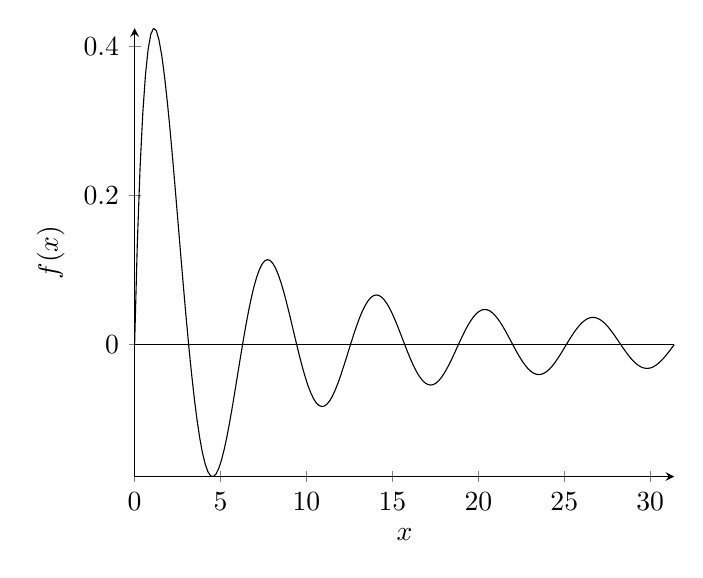
\begin{tikzpicture}
\begin{axis}[
    axis lines = left,
    xlabel = $x$,
    ylabel = {$f(x)$},
] 
\addplot [
    domain=0:31.4, 
    samples=200, 
    color=black,
]
{sin(deg(x))/(1+x)};
\addplot [
    domain=0:31.4, 
    samples=100, 
    color=black,
]
{0};
\end{axis}
\end{tikzpicture}
\end{enumerate}

\item Partition $[a,b]$ into small intervals $p: a = t_o < \ldots < t_n = b$. Let $M_i = \text{sup}\{f(x):x\in[t_{i-1},t_i]\}$, and $m_i = \text{inf}\{f(x):x\in[t_{i-1},t_i]\}$. Then sup$\{cf(x):x\in[t_{i-1},t_i]\}= c\cdot\text{sup}\{f(x):x\in[t_{i-1},t_i]\}= c\cdot M_i$. $\sum_{i=1}^ncM_i(t_i-t_{i-1})=c\sum_{i=1}^nM_i(t_i-t_{i-1})=cU(f,P)=U(cf,P)$. Then $\text{inf}\{U(cf,P):\text{all partitions P}\}=\text{inf}\{cU(f,P):\text{all partitions P}\}=c\cdot\text{sup}\{L(f,P):\text{all partitions P}\}=c\cdot I$, with $I=\text{inf}\{U(f,P):\text{all partitions P}\}$ Similarly, $\text{sup}\{L(cf,P):\text{all partitions P}\}=c\cdot S$. If $f$ is integrable over $[a,b]$, then $S=I\Rightarrow c\cdot S=c\cdot I=\int_a^bcf=c\int_a^bf$. 


\item \begin{enumerate}
    \item [(a)] $M_i=\text{sup}f_{[t_{i-1},t_i]}=1$ $\forall i$, and $m_i=\text{inf}f_{[t_{i-1},t_i]}=0$ $\forall i$. $U(f,P)=\sum_{i=1}^n1(t_i-t_{i-1})=1-0=1$. $L(f,P)=\sum_{i=1}^n0(t_i-t_{i-1})=0$. $S=\text{sup}\{L(f,P): \text{all P}\}=0$ and $I=\text{inf}\{U(f,P): \text{all P}\}=1$. $S\neq I$, so $f(x)$ is not integrable. 
    \item [(b)] $g$ clearly makes triangles of height $1$ and bases equal to $\frac{1}{2^n}$, $\forall n\in\mathbb{N}$. Therefore, the integral will be equal to the sum of all these triangles. The biggest triangle (the one formed from $\frac{1}{2}$ to $1$)is $\frac{\text{base}*\text{height}}{2}=\frac{\frac{1}{2}*1}{2}=\frac{1}{4}$, and the base of each triangle is reduced by half as you approach zero. Therefore, the integral will be equal to $\sum_{n=2}^\infty\frac{1}{2^n}=\frac{1}{2}$. 
\end{enumerate}


\item Let $f(x)=x^p$. Divide $[a,b]$ into an $n$ number of equal length partitions. Let $P_n:a=t_0<t_1<\ldots<t_n=b$, where $t_i=ac^{\frac{i}{n}}$, and $c=\frac{b}{a}$. 

If $p>1$ (and therefore $x^p$ is strictly increasing), then $M_i=\text{sup}f|_{[t_{i-1},t_i]}=f(t_i)=(ac^\frac{i}{n})^p$. If $1>p>0$, (and therefore $x^p$ is strictly decreasing), then $m_i=\text{inf}f|_{[t_{i-1},t_i]}=f(t_i)=(ac^\frac{i}{n})^p$. Either way, some Reimann sum will be $$R(f,P)=\sum_{i=1}^n(ac^\frac{i}{n})^p(ac^\frac{i}{n}-ac^\frac{i-1}{n})=a^{p+1}\sum_{i=1}^n(c^\frac{i(p+1)}{n}-c^\frac{ip+i-1}{n})$$ $\sum_{i=1}^n(c^\frac{i(p+1)}{n}-c^\frac{ip+i-1}{n})=\frac{(c^\frac{1}{n}-1)(c^{p+1}-1)c^\frac{p}{n}}{c^\frac{p+1}{n}-1}$. Taking the limit as $n\rightarrow\infty$, $\frac{(c^\frac{1}{n}-1)(c^{p+1}-1)c^\frac{p}{n}}{c^\frac{p+1}{n}-1}=\frac{c^{p+1}-1}{p+1}$. So $\int_a^b=a^{p+1}\frac{\frac{b}{a}^{p+1}-1}{p+1}=\frac{b^{p+1}-a^{p+1}}{p+1}$. 

\end{enumerate}

\end{document}
